\documentclass[tikz, border=15pt]{standalone}
\usetikzlibrary{shapes, arrows.meta, positioning, calc}

\begin{document}
	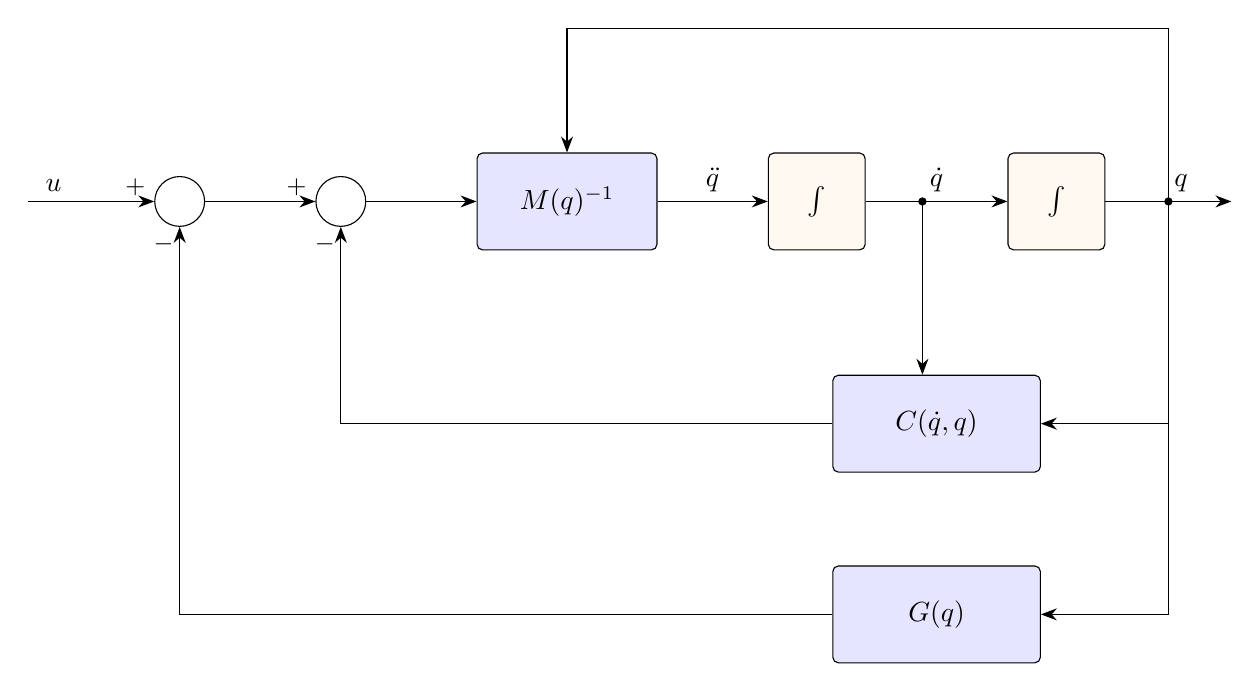
\begin{tikzpicture}[
		% --- ESTILOS DE LA SEGUNDA FIGURA ---
		block/.style = {draw, rectangle, minimum height=3.5em, minimum width=6.5em, align=center, rounded corners=2pt},
		int_block/.style = {draw, fill=orange!5, rectangle, minimum height=3.5em, minimum width=3.5em, align=center, rounded corners=2pt},
		sum/.style = {draw, fill=white, circle, minimum size=18pt, inner sep=0pt},
		>={Stealth[scale=1.2]}
		]
		
		% --- EJE PRINCIPAL ---
		\node [coordinate] (in) {};
		\node [sum, right=1.6cm of in] (sum1) {};
		\node [sum, right=1.4cm of sum1] (sum2) {};
		
		% Bloque M(q)^-1: Verde Pastel (Matriz de Inercia)
		\node [block, right=1.4cm of sum2, fill=blue!10] (mq) {$M(q)^{-1}$};
		
		% Integradores: Naranja Pastel (Bloques de la planta/estados)
		\node [int_block, right=1.4cm of mq] (int1) {\Large $\int$};
		\node [int_block, right=1.8cm of int1] (int2) {\Large $\int$};
		\node [coordinate, right=1.6cm of int2] (out) {};
		
		% --- BLOQUES DE RETROALIMENTACIÓN (Colores distintos y representativos) ---
		% Bloque C: Azul Pastel (Coriolis / Centrífugas)
		\node [block, minimum width=7.5em, fill=blue!10] (cq) at ($(int1.south)!0.5!(int2.south) + (0,-2.2)$) {$C(\dot{q}, q)$};
		% Bloque G: Rojo/Salmón Pastel (Gravitatorio)
		\node [block, minimum width=7.5em, fill=blue!10] (gq) at ($(cq.south) + (0,-1.8)$) {$G(q)$};
		
		% --- PUNTOS DE RAMIFICACIÓN ---
		\coordinate (branch_qdot) at ($(int1.east)!0.4!(int2.west)$);
		\coordinate (branch_q) at ($(int2.east)!0.5!(out)$);
		
		\fill (branch_qdot) circle (1.5pt);
		\fill (branch_q) circle (1.5pt);
		
		% --- CONEXIONES PRINCIPALES ---
		\draw [->] (in) -- node[above, pos=0.2] {$u$} (sum1);
		\draw [->] (sum1) -- (sum2);
		\draw [->] (sum2) -- (mq);
		\draw [->] (mq) -- node[above, midway] {$\ddot{q}$} (int1);
		\draw [->] (int1) -- node[above, midway] {$\dot{q}$} (int2);
		\draw [->] (int2) -- node[above, pos=0.6] {$q$} (out);
		
		% --- LAZOS DE RETROALIMENTACIÓN ---
		
		% Lazo superior hacia M(q)^-1
		\draw [->] (branch_q) -- ++(0,2.2) -| (mq.north);
		
		% Lazo desde q_dot hacia C (SOLUCIÓN: Descenso 100% vertical libre de curvaturas o escalones)
		\draw [->] (branch_qdot) -- (branch_qdot |- cq.north);
		
		% Lazos desde q hacia el lateral de C y G
		\draw [->] (branch_q) |- (cq.east);
		\draw [->] (branch_q) |- (gq.east);
		
		% Retornos ortogonales a los sumadores
		\draw [->] (cq.west) -| (sum2.south);
		\draw [->] (gq.west) -| (sum1.south);
		
		% --- SIGNOS DE LOS SUMADORES ---
		% Sumador 1
		\node[above left, inner sep=2pt, xshift=-1pt] at (sum1.west) {\small $+$};
		\node[below left, inner sep=2pt, yshift=-1pt] at (sum1.south) {\small $-$};
		
		% Sumador 2
		\node[above left, inner sep=2pt, xshift=-1pt] at (sum2.west) {\small $+$};
		\node[below left, inner sep=2pt, yshift=-1pt] at (sum2.south) {\small $-$};
		
	\end{tikzpicture}
\end{document}